\documentclass[]{article}
\usepackage{graphicx}
\usepackage{float}
\usepackage{enumitem}
\usepackage{hyperref}
\hypersetup
{
	colorlinks=true,
	citecolor=black,
	filecolor=black,
	linkcolor=black,
	urlcolor=blue,
	linktoc=all,
	linkcolor=black,
}

\setlist{nosep}
\graphicspath{ {images/} }

% Title Page
\title{Department Of Computer Science Advising Tool \\ User Manual}
\author{Brian Hooper, Nick Rohde, Rico Adrian \\ Central Washington University}
\date{Last Updated: March 8th, 2018}

\begin{document}
\maketitle
\tableofcontents


\pagebreak\section{Introduction}
	
\includegraphics[width=\textwidth]{computer_science_logo.png}
	\subsection{Description}\label{ssec:1}
	
		The Computer Science Student Advising Tool is a website for use by Student Advisors within the Department of Computer Science at Central Washington University. The tool provides a secure interface for automating the generation of student graduation plans based off of degree requirement and course catalog information. Functionality provided by the tool includes loading and saving student graduation plans, modifying student graduation plans, automatic scheduling of graduation plans, as well as modification of course, degree, and user information. 
	\subsection{Purpose}\label{ssec:2}
	
		The purpose is of this document is to provide a thorough explanation of how to use all functionality provided by the Advising Tool for the Department of Computer Science at Central Washington University. 
	\subsection{General Functionality}\label{ssec:3}
	
		The application consists of a login interface, advising interface, and a set of database management tools for managing Course, Degree, and User data. The tool can be accessed from within the Department of Computer Science network via its domain name:
		\begin{center}
			http://cs-advising.cs.cwu.edu/
		\end{center}

\pagebreak\section{Getting started}
	\subsection{Authenticating}\label{ssec:4}
	
		The home page for the website consists of a simple login interface, as well as a status message that displays the connection to the database. To access the site, simply log in by entering your Username and Password into the input boxes within the "Login" box. Both the Username and Password are case-sensitive, and an error message will be displayed if the either the Username or Password do not match, or if there is nothing entered in the text field. For information on obtaining a user account or resetting your password, consult section \ref{ssec:14} "Managing User Accounts"
	\subsection{Authentication Levels}\label{ssec:16}
	
		The website provides two levels of authentication, "Advisor" accounts and "Administrator" accounts. For Advisor accounts, access to the Advising page is provided to create, save, and modify student graduation plans, but access to the database manipulation tools including Course, Degree, and User management is not provided. Administrator accounts are provided access to all aspects of the application, including all functionality provided to Advisor accounts, as well as access to Course, Degree, and User management pages.
	\subsection{Navigation}\label{ssec:15}
	
		Once authenticated, the user will be redirected to either the "Advising" interface, or the "Course Management" interface, depending on the user's level of authentication. To navigate to different sections of the website, a menu is provided near the top right of the page. The links to pages that are included in the menu correspond to the pages that the user is able to access with their current authentication level. For advisors, only a link to the "Advising" page is provided. For administrators, links to Advising, Course Management, Degree Management, and User Management are provided.\\
		\begin{figure}[h]
			\caption{Navigation menu}
			\centering
			
\includegraphics[width=\textwidth]{navigation.PNG}
		\end{figure}

\pagebreak\section{Generating Graduation Plans}
	\subsection{Functionality}\label{ssec:6}
	
		The primary purpose of the advising tool is to generate student graduation plans. The Advising page of the website provides an interface for both loading existing graduation plans, as well as creating new graduation plans. 
	\subsection{Creating and Loading Student Plans}\label{ssec:7}
	
		To access the graduation plan management page, a graduation plan must be loaded from the database. If a student plan already exists, the user may load the plan by entering the student's unique ID into the input field of the "Load Existing Student Plan" dialog box, found on the Advising page and shown here in figure \ref{loadstudent}. \\
		\begin{figure}[H]
			\caption{Load Student Dialog Box}
			\label{loadstudent}
			\centering
			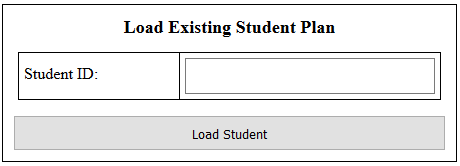
\includegraphics{loadstudent.PNG}
		\end{figure}
	
		If a student plan does not already exist in the database, it must be created. To create a student, enter their full name, unique student ID, starting quarter, and degree from the "Create New Student Plan" dialog box shown in figure \ref{createstudent}.

		Care should be taken to ensure that the student ID field is correct, as this unique value is needed to load the student's graduation plan once it is stored in the database. Furthermore, creating a new student plan while using an existing student ID will overwrite any previous records stored using that ID. \\~\\
	
		The "Starting quarter" field should reflect the first academic quarter that the student will enroll in courses at Central Washington University. The "Degree" field determines the list of graduation requirements that will be added to the student plan. For each degree, both the academic catalog year and specific degree name are shown. For example, for the information entered in the dialog box shown in figure \ref{createstudent}, a student will be created for student "John Smith", with unique ID "123456", and a graduation plan for that student will be created containing a single, empty "Fall 2017" Quarter, and a list of unmet Degree Requirements from the "Bachelor of Science - Computer Science" degree requirements for Academic Catalog year 2017-2018.
		\begin{figure}[H]
			\caption{Create Student Dialog Box}
			\label{createstudent}
			\centering
			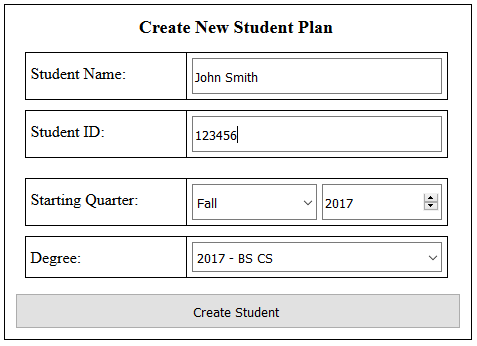
\includegraphics{createstudent.PNG}
		\end{figure}
	\subsection{Modifying a Student Plan}\label{ssec:8}
	
		When a graduation plan is loaded, the user is redirected to the graduation plan management page, shown in figure \ref{planmanagement}. A graduation plan consists of a list of Quarters, each containing a title, list of courses, and number of credits. In the example shown in figure \ref{planmanagement}, the quarter "Fall 2018" contains courses (displayed using their abbreviated course ID), "University 101", "Math 153", "English 101", and "Computer Science 110". 
		\begin{figure}[H]
			\caption{Graduation Plan Management}
			\label{planmanagement}
			\centering
			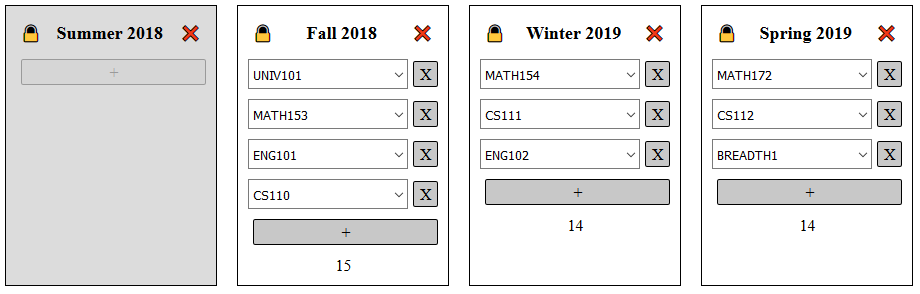
\includegraphics[width=\textwidth]{planmanagement.PNG}
		\end{figure}
		\begin{figure}[H]
			\caption{Graduation Plan Management}
			\label{quarter}
			\centering
			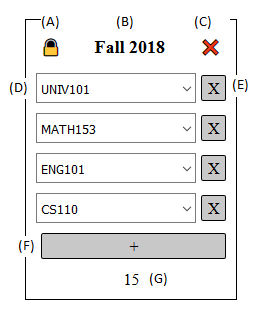
\includegraphics{quarter.PNG}
		\end{figure}
		Each Quarter contains a the following items, as shown in figure \ref{quarter}:
		\begin{itemize}
			\item (A) Lock Button
			\item (B) Quarter Title
			\item (C) Delete Quarter Button
			\item (D) Select Course Drop-Down
			\item (E) Remove Course Button
			\item (F) Add Course Button
			\item (G) Total Credits
		\end{itemize}
		
		\pagebreak 
		(A) The Lock Button allows a user to force the scheduling algorithm to ignore that particular quarter. This is useful for when a student does not want to take courses during a specific quarter, or when a student wishes to take a lighter course load than their maximum number of credits. The quarter lock can also be used to selectively take courses in some summer quarters, but not all. When a quarter is locked, the quarter is colored dark gray. An example of a locked quarter "Summer 2018" is shown in figure \ref{planmanagement}.\\~\\
		
		(B) The Quarter Title contains the Season (Summer, Fall, Winter, or Spring) and the year for that quarter, and cannot be changed. To modify a student's starting quarter, the user should overwrite the student's graduation plan by creating a new student using the same unique ID. For more information on creating students, see section \ref{ssec:7}.\\~\\
		
		(C) The Delete Quarter Button removes all Courses from that quarter, and adds each course into the list of unmet requirements. If a quarter is the last quarter in the student's schedule, the quarter object is also removed. If it is not, the quarter is simply left with no courses, to preserve the ordering of the quarters. \\~\\
		
		(D) The Select Course drop-down represents a single course in the quarter. The drop-down list can be swapped with another course in the student's unmet requirements, provided that the course is offered during that particular quarter. In that case, the original course will be added back into the student's list of unmet requirements.\\~\\
		
		(E) The Remove course button removes a course from that quarter, and adds the course back into the list of unmet requirements. If there is no course selected, the drop-down list is simply removed.\\~\\
		
		(F) The Add Course button adds another drop-down list to the quarter, populated with all courses in the unmet requirements list that are offered during that particular quarter. \\~\\
		
		(G) The Total Credits displays the sum of all course credits taken during the quarter. If the total number of credits is higher than the students specified maximum number of credits, the number is highlighted in red to show to the advisor that a signature from the department chair must be obtained to allow the student to take a higher course load than their specified maximum.
	\subsection{Unmet Requirements}\label{ssec:17}
		\begin{figure}[H]
			\caption{A blank quarter with unmet requirements}
			\label{unmetrequirements}
			\centering
			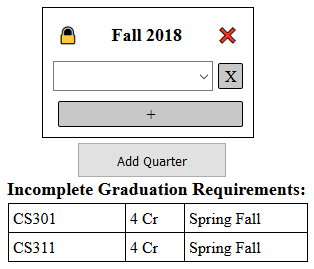
\includegraphics{unmetrequirements.PNG}
		\end{figure}
		
		When a new student is added to the application, they are given a single, blank starting quarter, and a list of unmet requirements. This list of unmet requirements is passed to the scheduling algorithm when generating a graduation plan. For information on the scheduling algorithm, see section \ref{ssec:10}. As courses are added to quarters, they are removed from the list of unmet graduation requirements. If all requirements are completed, the message "All requirements completed!" is displayed. Each row in the list of unmet requirements consists of information from three Columns: Course ID, Number of Credits, and Quarters offered. The Course ID is the unique identifier for the course used to manage courses in the database. \\~\\

		Just above the unmet requirements list is the "Add Quarter" button. This button appends a new, blank quarter to the end of the student's schedule. For example, if the last quarter in a student's schedule is "Fall 2018", the Add Quarter button would add an additional "Winter 2019" quarter just after "Fall 2018". This button can be used to create an entire student schedule from a list of unmet requirements and a single starting quarter.
	\subsection{Working with the Base Case}\label{ssec:9}
		To save time when creating multiple similar graduation plans, a "Base Case" can be loaded to fill in a student's schedule with a standard graduation plan. After the base case is loaded, modifications can be made to suite the students individual needs. When the "Load Base Case" button (shown in figure \ref{basecasebutton}) is pressed, a confirmation is shown asking the user if they are sure that they want to load the base case. Care should be taken that this feature is not evoked accidentally, as it will overwrite any unsaved changes that have been applied to the student plan. A "Save Base Case" button is also provided to save the current schedule as the base case, in the event that the base case should be updated. 
		\begin{figure}[H]
			\caption{A blank quarter with unmet requirements}
			\label{basecasebutton}
			\centering
			
\includegraphics{basecasebutton.PNG}
		\end{figure}
	\subsection{Using the Scheduling Algorithm}\label{ssec:10}
		The purpose of the scheduling algorithm is to automatically place unmet requirements into a students schedule. The algorithm is designed to return the schedule that takes the least number of quarters to complete. Prerequisite courses, minimum and maximum quarterly credits, locked quarters, and whether or not the student is able to take summer courses, are all taken into consideration by the scheduling algorithm. \\~\\
		
		When the "Generate" button is pressed, shown at the bottom of figure \ref{algorithmbutton}, the student's schedule, including all courses that have been added to quarters, is passed to the scheduling algorithm, along with the list of unmet requirements and the content of the "Constraints" dialog box (Fig. \ref{algorithmbutton}). It is important to note that the algorithm does not change any courses that are already added to quarters, regardless of whether or not they meet the student's specific constraints.\\~\\
		
		 The "Constraints" box consists of three fields: "Minimum Credits", "Maximum Credits", and "Taking Summer Courses". The "Minimum Credits" field designates the smallest number of credits that a student can take during an individual quarter. If the algorithm attempts to create a plan that gives a student a quarter that does not meet the minimum credits, that plan is discarded in favor of a plan that meets that constraint. Likewise, the "Maximum Credits" field does not allow the scheduling algorithm to add courses to a plan that will result in that quarter having a greater number of credits than the students defined maximum. Finally, the "Taking Summer Courses" determines if the algorithm is able to add courses to summer quarters. If the "Taking Summer Courses" button is checked, any summer quarters that have been locked are still prohibited from having courses added to them.\\~\\
		
		Once the "Generate" button is pressed, it may take some time (a few seconds) to find the best schedule from the parameters it is given. A dialog box is shown that will automatically close when the algorithm is complete, after which the displayed schedule will be updated with the results of the computation. 
		\begin{figure}[H]
			\caption{Constraints and controls for evoking the scheduling algorithm}
			\label{algorithmbutton}
			\centering
			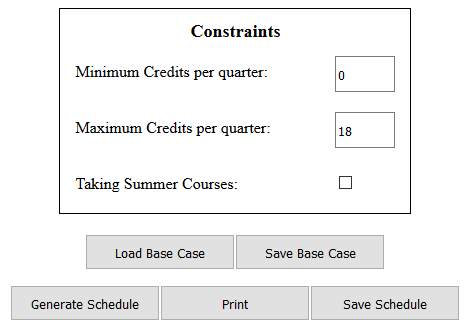
\includegraphics{schedulingalgorithm.PNG}
		\end{figure}
	\subsection{Other Graduation Plan Functionality}\label{ssec:11}
		Once the student's schedule is complete, the plan can be saved to the database by clicking the "Save Schedule" button, shown in figure \ref{algorithmbutton}. A "Print" button is also provided to format the schedule for printing on standard 8.5" by 11" paper. The "Print" button automatically saves the student schedule when it is pressed. 
\pagebreak\section{Database Management}
	\subsection{Overview}\label{ssec:18}
		To create and modify student plans, the user must be able to manage the course and degree information stored in the database. A set of tools have been provided to manage this information, as well as an interface for managing user accounts. To access the database management pages, a user must have administrator access. 
	\subsection{Managing Courses}\label{ssec:12}
		The Manage Courses page provides an interface for creating, removing, and modifying the courses stored in the database. Search functionality is provided to quickly find a specific course to modify or remove. The Course Search Dialog (shown in figure \ref{searchcourses}) allows the user to select courses by course number, department, or quarters offered. \\~\\
		
		The Course Number field will restricts the search result from displaying courses that are outside the bounds provided by the user. To select a course with a specific course number, the minimum and maximum can be set to equal each other. In figure \ref{searchcourses}, the minimum course number is set to 0, and the maximum course number is set to 999. \\~\\
		
		The department drop-down allows users to display courses from a specific department. If the "--- Any ---" option is selected, courses are displayed from all departments. When a new department is added, this drop-down list is automatically updated. \\~\\
		
		The Courses Offered option boxes displays only courses that are offered during the quarters which are selected. Whether or not a course is taken during a quarter that is not selected is not taken into consideration. For example, if a course is offered in Winter, it will be displayed when "Winter" is checked, regardless of whether or not it is offered any other quarters. In the example shown in figure \ref{searchcourses}, the result will display all courses offered in fall, all courses offered in winter, and all courses offered in spring, but not any courses that are offered exclusively in summer.
		\begin{figure}[H]
			\caption{Course Search Dialog}
			\label{searchcourses}
			\centering
			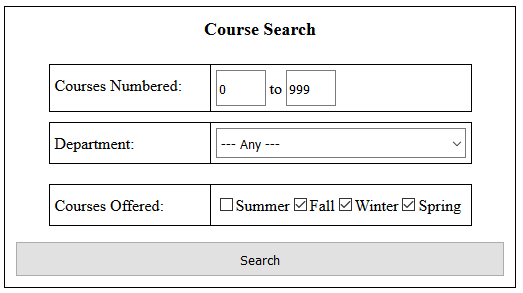
\includegraphics{coursesearch.PNG}
		\end{figure}
		\begin{figure}[H]
			\caption{Course Search Results}
			\label{coursedisplay}
			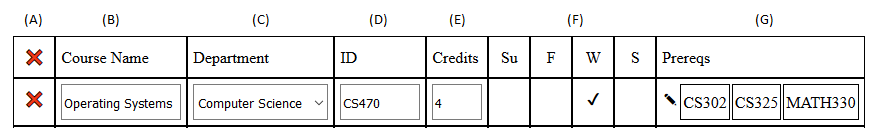
\includegraphics[width=\textwidth]{coursedisplay.PNG}
		\end{figure}
		When the "Search" button is pressed, all courses matching the search criteria are displayed to the user. The following information is displayed for each course:
		\begin{itemize}
			\item (A) Delete Button
			\item (B) Course Name
			\item (C) Department
			\item (D) Course ID
			\item (E) Number of credits
			\item (F) Quarters Offered
			\item (G) Prerequisite Courses
		\end{itemize}~\\
		
		(A) The Delete button is used to remove a course from the database. If the row contains an entry in the ID column, a confirmation dialog will be shown to prompt the user if they want to delete the course. If a course is accidentally deleted, it can be restored by simply refreshing the page without saving the changes. \\~\\
		
		(B) The Course name should be the long title of the course. In the example shown in figure \ref{coursedisplay}, the course name is "Operating Systems". The course name is not used by the scheduling algorithm, but should be descriptive enough that any users modifying the course information can understand what course the row refers to.\\~\\
		
		(C) The Course Department is a drop-down list that can be used to specify which the department for a specific course. When a new department is added, each drop-down box is automatically updated. The department field is not used by the scheduling algorithm, but is useful when using the search courses function. \\~\\
		
		(D) The Course ID is the unique identifier for the course. This is the value that is used by the scheduling algorithm and plan management pages, so care should be taken to ensure that the value is correct. If a course is added with a course ID that already exists, the previous course will be overwritten. \\~\\
		
		(E) The Credits field determines the number of credits. It should be given as a positive integer. \\~\\
		
		(F) The Quarters Offered field is presented as a series of four check boxes. To specify that a course is offered a specific quarter, simply check the corresponding box. If no quarter is selected, the course will not be saved to the database.\\~\\
		
		(G) The Prerequisite Courses box contains the prerequisite courses for the course. By clicking on the Prerequisite Courses box, a pop-up dialog box is displayed (shown in figure \ref{prereqs}). The Prerequisite Popup box displays a course search interface similar to the search interface used to search for courses, as well as a list of prerequisite courses. Courses that are currently included as a prerequisite are shown at the bottom of the screen, and can be removed as a prerequisite by clicking on the large X to the left of the course ID. Courses returned by the search are displayed immediately below the search box, and can be added as a prerequisite by clicking on the large check mark to the left of the course ID. The course can be updated by clicking the "Save" button, or the prerequisite update can be canceled by clicking either the "Close" button at the bottom of the Prerequisite popub box or the "X" button on the top right corner of the Prerequisite popup box. It is important to note that when the "Save" button in the prerequisite dialog is pressed, the changes to the course are not saved to the database until the "Save Changes" button is pressed at the bottom of the Manage Courses page. \\~\\
		\begin{figure}[H]
			\caption{Prerequisite Popup Box}
			\label{prereqs}
			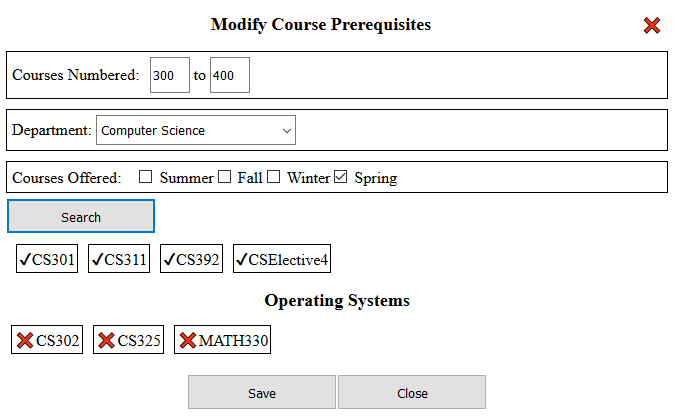
\includegraphics[width=\textwidth]{prereqs.PNG}
		\end{figure}
	
		New Courses can be added by pressing the "Add New Course" button at the bottom of the Manage Courses page (shown in figure \ref{addepartment}). When the "Add New Course" button is pressed, a new row is appended to the course search results, with all values set to blank. If the "Save Changes" button is pressed before a course ID has been entered into the ID field, the course will not be saved. It is recommended to save after each new course created. If the "Search" button is pressed before the new course has been saved, it will be lost. \\~\\
		
		New Departments can be added by pressing the "Add Department" button, shown in figure \ref{addepartment}. When this button is pressed, a dialog box is shown asking for the name of the new department. When a name is provided, that value is added to each "Department" select drop-down list on the page. If there are no courses that contain a department, then that department is removed from the database. 
		\begin{figure}[H]
			\caption{Course Management Buttons}
			\label{addepartment}
			\centering
			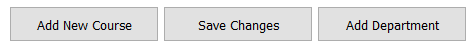
\includegraphics{savecourses.PNG}
		\end{figure}
	\subsection{Managing Degree Requirements}\label{ssec:13}
		The Manage Degrees page provides an interface for modifying the lists of degree requirements that are stored in the database. The user can either create a new degree by using the "Create New Degree" dialog box (shown in figure \ref{createdegree}), or modify an existing degree by using the "Load Degree" dialog box (shown in figure \ref{loaddegree}).
		\begin{figure}[H]
			\caption{Create Degree Dialog}
			\label{createdegree}
			\centering
			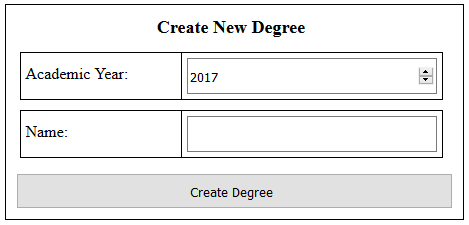
\includegraphics{createdegree.PNG}
		\end{figure}
		\begin{figure}[H]
			\caption{Load Degree Dialog}
			\label{loaddegree}
			\centering
			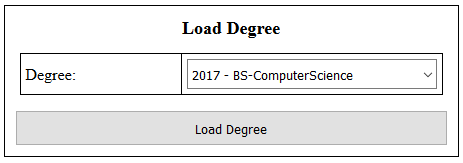
\includegraphics{loaddegree.PNG}
		\end{figure}
		To create a new degree, choose an integer academic year for the degree, and a unique degree name. If a degree is already stored in the database with that name, it will be overwritten. The academic year should be the first year for an academic catalog. For example, for the Bachelor of Science in Computer Science degree for the 2017 - 2018 academic catalog, the values "2017" and "BS-ComputerScience" should be chosen. Spaces should not be included in the degree name. To load an existing degree, simply choose the name of the degree from the drop-down list in the "Load Degree" box and press "Load Degree".\\~\\
		\begin{figure}[H]
			\caption{Degree Results Dialog}
			\label{degreeresults}
			\centering
			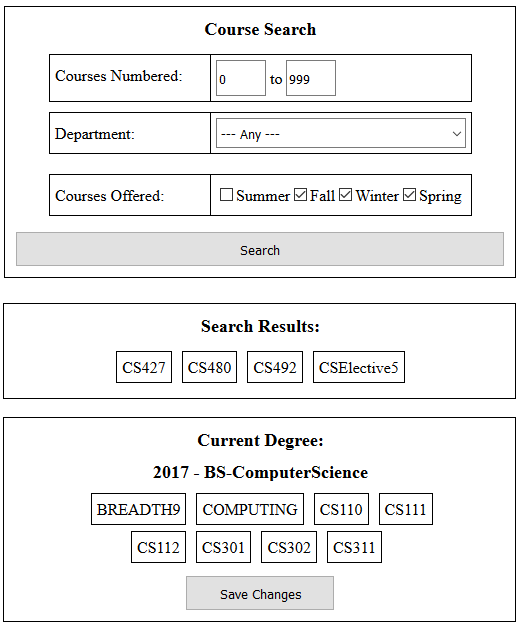
\includegraphics{degreeresults.PNG}
		\end{figure}
		Similar to the functionality provided by the Manage Courses page, a search dialog is provided to easily select courses to add or remove to a degree. The "Search Results" box contains the courses fit the given search criteria, and the "Current Degree" box contains courses that are listed as a requirement for a current degree. Clicking on a course in the "Search Results" box will add the course to the current degree requirements, provided it is not already included. Clicking on a course in the "Current Degree" box will remove a course from the current degree requirements. Finally, the "Save Changes" button writes the changes to the database. 
		
	\subsection{Managing User Accounts}\label{ssec:14}
		A "Manage Users" page is provided for administrators to create, modify, and delete users. An Advisor that does not have administrator privileges may change their password by clicking the "[ Change Password ]" button near the top left corner of the screen. Administrators may add a new user account, delete a user account, change whether or not a user is an administrator or is activated, and change a users password. The "User Management" page (shown in figure \ref{manageusers}) displays all user accounts in a list. A user can be deleted by clicking on the X button to the left of the user's username. Administrator and Active status can be changed by toggling the buttons in their respective columns. If a user is set to inactive, their account will still exist on the system, but they will be unable to log in. A user's password can be reset by clicking on the "Change PW" button to the right of the Administrator and Active buttons. 
		\begin{figure}[H]
			\caption{Manage Users List}
			\label{manageusers}
			\centering
			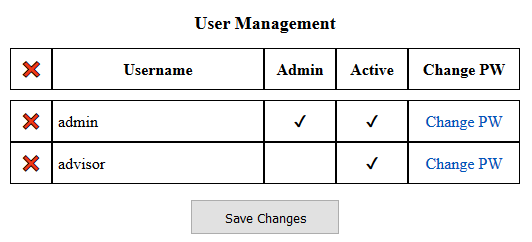
\includegraphics[width=\textwidth]{manageusers.PNG}
		\end{figure}
		New user accounts can be added by entering a username and password into the "Add User" dialog box, shown in figure \ref{adduser}. If the username is already taken, or if the passwords do not match, the update will be rejected.
		\begin{figure}[H]
			\caption{Add Users Box}
			\label{adduser}
			\centering
			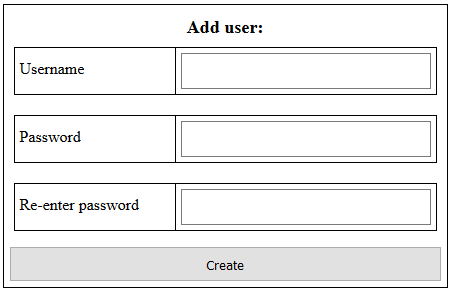
\includegraphics{adduser.PNG}
		\end{figure}
		To change a password, a user can click on the "Change Password" link on the top left corner of the screen, or an administrator can change a specific users password by clicking on the "Change PW" button on the right side of the "Manage Users" page. The user will then be redirected to "Change Password" page (seen in figure \ref{changepassword}, where the user will be prompted to enter their old password, and provide a new password. An administrator can change another users password by leaving the old password field blank. 
		
		\begin{figure}[H]
			\caption{The Change Password Dialog Box}
			\label{changepassword}
			\centering
			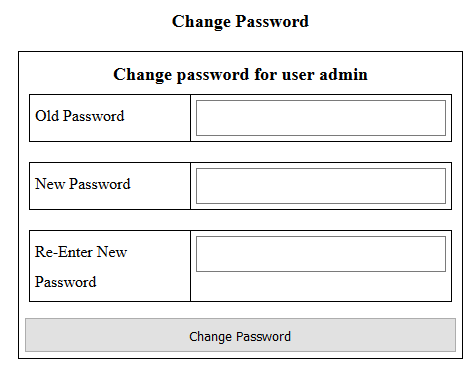
\includegraphics{changepassword.PNG}
		\end{figure}
\end{document}          
